\documentclass{standalone}
\usepackage{pgfplots}
\pgfplotsset{compat=1.13}
\usepackage{amsmath}
\colorlet{paleBlue}{blue!10!white}

\begin{document}

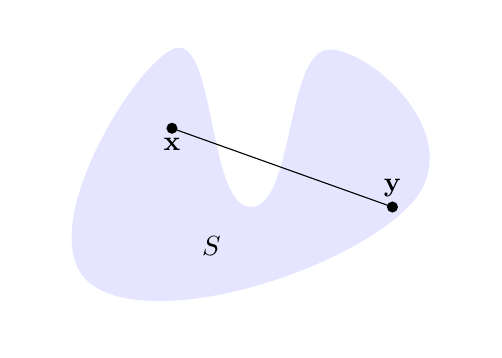
\begin{tikzpicture}
    \fill[paleBlue] plot [smooth cycle, tension=1] coordinates {(0,0) (1,3) (2,1) (3,3) (4,1)};
    \fill[black] (1,2) circle (2pt) node[below]{\(\mathbf{x}\)};
    \fill[black] (3.8,1) circle (2pt) node[above]{\(\mathbf{y}\)};
    \draw[] (1,2) -- (3.8,1);
    \node at (1.5,0.5){\(S\)};
\end{tikzpicture}

\end{document}